% chktex-file 44

\section{\large Ejercicio 4. Rango de una Matriz.}

Determinar el rango de la matriz dada, utilizando el método de Gauss-Jordán y el método de los determinantes.

\[
    C=\left(
        \begin{array}{ccc}
            3 & 0 & 3 \\
            1 & 6 & -1 \\
            2 & 2 & 2 \\
            0 & -1 & 1 \\
        \end{array}
    \right)
\]

\textbf{Método de Gauss-Jordán:}
\[
    \begin{aligned}
        \left(
            \begin{array}{ccc|c}
                3 & 0 & 3 & 0 \\
                1 & 6 & -1 & 0 \\
                2 & 2 & 2 & 0 \\
                0 & -1 & 1 & 0 \\
            \end{array}
        \right)
        &f1/3 \\ \\
        \left(
            \begin{array}{ccc|c}
                1 & 0 & 1 & 0 \\
                1 & 6 & -1 & 0 \\
                2 & 2 & 2 & 0 \\
                0 & -1 & 1 & 0 \\
            \end{array}
        \right)
        &-1f1+f2 \\ \\
        \begin{aligned}
            -1f1+f2=
            &\begin{array}{ccc|c}
                -1 & 0 & -1 & 0 \\
                1 & 6 & -1 & 0 \\
                \hline
                0 & 6 & -2 & 0 \\
            \end{array}
        \end{aligned} \\ \\
        \left(
            \begin{array}{ccc|c}
                1 & 0 & 1 & 0 \\
                0 & 6 & -2 & 0 \\
                2 & 2 & 2 & 0 \\
                0 & -1 & 1 & 0 \\
            \end{array}
        \right)
        &-2f1+f3 \\ \\
        \begin{aligned}
            -2f1+f3=
            &\begin{array}{ccc|c}
                -2 & 0 & -2 & 0 \\
                2 & 2 & 2 & 0 \\
                \hline
                0 & 2 & 0 & 0 \\
            \end{array}
        \end{aligned} \\ \\
        \left(
            \begin{array}{ccc|c}
                1 & 0 & 1 & 0 \\
                0 & 6 & -2 & 0 \\
                0 & 2 & 0 & 0 \\
                0 & -1 & 1 & 0 \\
            \end{array}
        \right)
        &f2/6
    \end{aligned}
\]

\[
    \begin{aligned}
        \left(
            \begin{array}{ccc|c}
                1 & 0 & 1 & 0 \\
                0 & 1 & -\frac{1}{3} & 0 \\
                0 & 2 & 0 & 0 \\
                0 & -1 & 1 & 0 \\
            \end{array}
        \right)
        &-2f2+f3 \\ \\
        \begin{aligned}
            -2f1+f3=
            &\begin{array}{ccc|c}
                0 & -2 & \frac{2}{3} & 0 \\
                0 & 2 & 0 & 0 \\
                \hline
                0 & 0 & \frac{2}{3} & 0 \\
            \end{array}
        \end{aligned} \\ \\
        \left(
            \begin{array}{ccc|c}
                1 & 0 & 1 & 0 \\
                0 & 1 & -\frac{1}{3} & 0 \\
                0 & 0 & \frac{2}{3} & 0 \\
                0 & -1 & 1 & 0 \\
            \end{array}
        \right)
        &f2+f4 \\ \\
        \begin{aligned}
            f2+f4=
            &\begin{array}{ccc|c}
                0 & 1 & -\frac{1}{3} & 0 \\
                0 & -1 & 1 & 0 \\
                \hline
                0 & 0 & \frac{2}{3} & 0 \\
            \end{array}
        \end{aligned} \\ \\
        \left(
            \begin{array}{ccc|c}
                1 & 0 & 1 & 0 \\
                0 & 1 & -\frac{1}{3} & 0 \\
                0 & 0 & \frac{2}{3} & 0 \\
                0 & 0 & \frac{2}{3} & 0 \\
            \end{array}
        \right)
        &\frac{f3}{\frac{2}{3}} \\ \\
        \left(
            \begin{array}{ccc|c}
                1 & 0 & 1 & 0 \\
                0 & 1 & -\frac{1}{3} & 0 \\
                0 & 0 & 1 & 0 \\
                0 & 0 & \frac{2}{3} & 0 \\
            \end{array}
        \right)
        &-\frac{2}{3}f3+f4 \\ \\
        \begin{aligned}
            -\frac{2}{3}f3+f4=
            &\begin{array}{ccc|c}
                0 & 0 & -\frac{2}{3} & 0 \\
                0 & 0 & \frac{2}{3} & 0 \\
                \hline
                0 & 0 & 0 & 0 \\
            \end{array}
        \end{aligned} \\ \\
    \end{aligned}
\]

\[
    \left(
        \begin{array}{ccc|c}
            1 & 0 & 1 & 0 \\
            \cmidrule{1-1} \multicolumn{1}{c|}{0} & 1 & -\frac{1}{3} & 0 \\
            \cmidrule{2-2} 0 & \multicolumn{1}{c|}{0} & 1 & 0 \\
            \cmidrule{3-3} 0 & 0 & 0 & 0 \\
        \end{array}
    \right)
\]

\[
    Rang(C)=3
\]

\textbf{Método de los determinantes:}

\begin{itemize}
    \item Comprobamos el rango máximo que es tres, tomando 3 columnas de la matriz.
    \[
        \begin{vmatrix}
            3 & 0 & 3 \\
            1 & 6 & -1 \\
            2 & 2 & 2 \\
        \end{vmatrix}
        = 36+6-(36-6)=36+6-30=12\neq0
    \]
    \[
        Rang(C)=3
    \]
\end{itemize}

\begin{figure}[ht!]
    \centering
    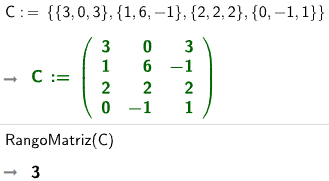
\includegraphics[width=200pt,height=150pt]{img/imagen12.png}
    \caption{Comprobación en GeoGebra}
\end{figure}

\textbf{Solución: }Debido a que al realizar la matriz escalonada una de las cuatro filas es nula y además al calcular la determinante de una de las tres filas de la matriz el resultado es diferente de cero, entonces el rango es 3.